\documentclass[a4paper, 11pt, spanish]{article}

% ---------------- Paquetes de formato.
\usepackage[spanish]{babel} % Para codificar el texto.
\usepackage[top=70mm, bottom=30mm, left=18mm, right=18mm]{geometry} % Para modificar el tamaño de las hojas.
\usepackage{fancyhdr} % Para poner la institución, dpto y curso arriba.
\usepackage{parallel} % Para escribir en columnas (Poner los integrantes a la derecha).
\usepackage[firstpage=false]{background} % Para poner el logo de la U arriba en todas las páginas.
\usepackage{enumerate} % Para poder enumerar como a), b), etc.
\usepackage[utf8]{inputenc} % Para usar acentos en vez de \'.

% ---------------- Paquetes graficos.
\usepackage{graphicx} % remove the demo option.
\usepackage{tikz}
\usepackage{caption}
\usepackage{subcaption} % Para usar sub-figuras

% ---------------- Paquetes matematicos.
\usepackage{amsmath} % Para poder hacer N^o y se vea bonito.
\usepackage{amsthm} % Fonts matematicos.
\usepackage{amssymb} % Para usar \therefore
\usepackage{commath} % Para usar \abs y \norm

% ---------------- Paquetes 'computines'.
\usepackage{listings} % Para escribir codigo y que se vea bonito.
\usepackage[% Descomentar las opciones a usar.
spanish,
%boxed, % Encierra los algoritmos en un cuadro.
boxruled, % Encierra los algoritmos en un cuadro colocando el titulo al comienzo.
%ruled, % Coloca una linea al comienzo y otra al final del algoritmo. El titulo de este queda al comienzo del algoritmo.
%algoruled, % Lo mismo que el anterior pero mas espaciado.
%tworuled, % Como ruled pero sin una linea al comienzo.
%algochapter, % Los algoritmos se enumeran segun capitulo.
%algopart, % Los algoritmos se enumeran por partes.
%figure, % Los algoritmos son considerados figuras (y por ende salen en \listoffigures).
%linesnumbered, % Enumera las lineas.
longend % Los end son para cada ciclo, por ejemplo endif para los if-else.
]{algorithm2e}

% ---------------- Paquetes miscelaneos.
%\usepackage{lipsum} % Para hacer placeholders.
\usepackage{bohr} % Para dibujar atomos.

% ---------------- Comando mas corto para insertar figuras. Ojo que deben estar guardadas en ./img/
% \fig{name}{width}{height}{caption}
\newcommand{\fig}[4]{%
	\begin{figure}[!ht]
		\centering
		\includegraphics[width=#2, height=#3]{img/#1}
		\caption{#4}
	\end{figure}
}
% ejemplo:
%			\fig{nombre_imagen.png}{10cm}{5cm}{Titulo de la imagen}


%\begin{figure}[!ht]
%\centering
%\begin{subfigure}{.5\textwidth}
%  \centering
%  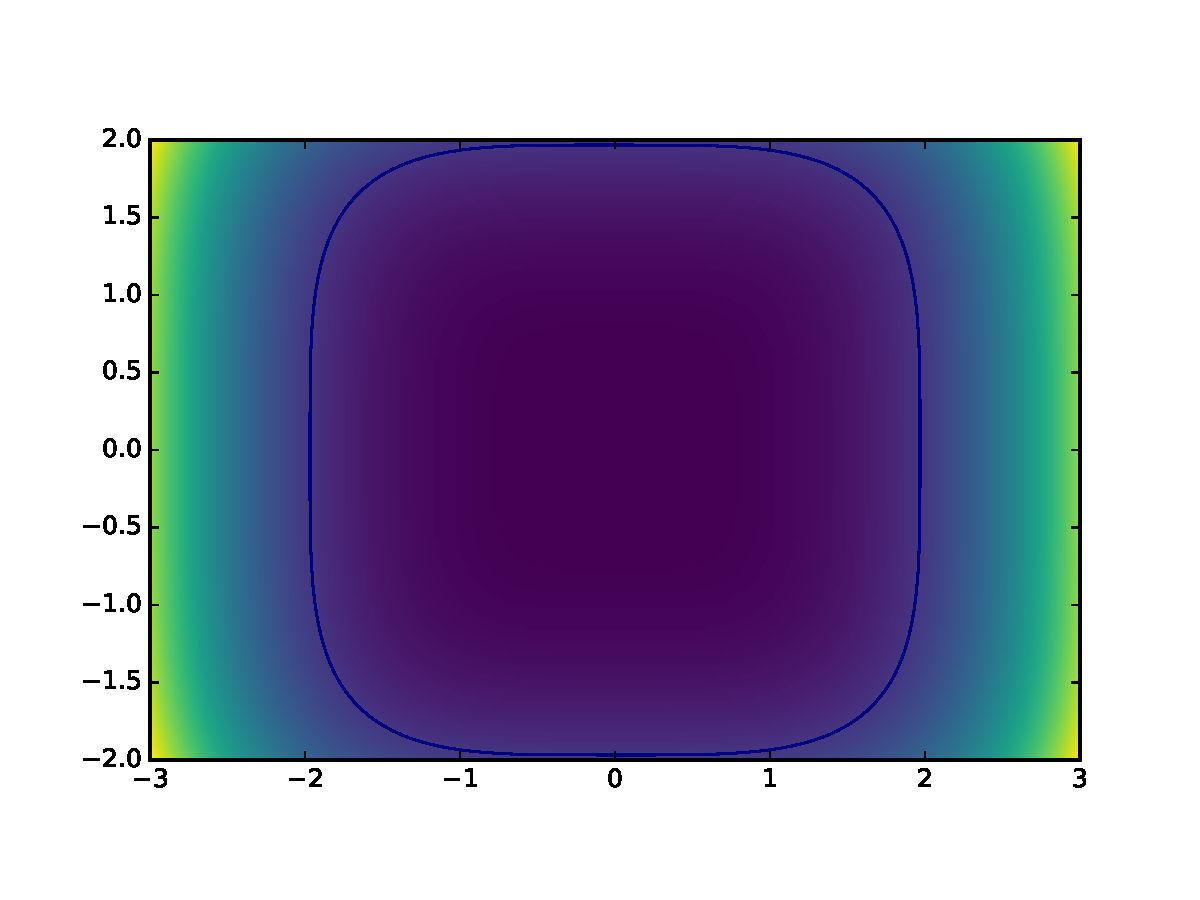
\includegraphics[width=10cm, height=8cm]{img/curva0f1.pdf}
%  \caption{Curva de nivel 0 de $F_{1}$.}
%  \label{fig:sub1}
%\end{subfigure}%
%\begin{subfigure}{.5\textwidth}
%  \centering
%  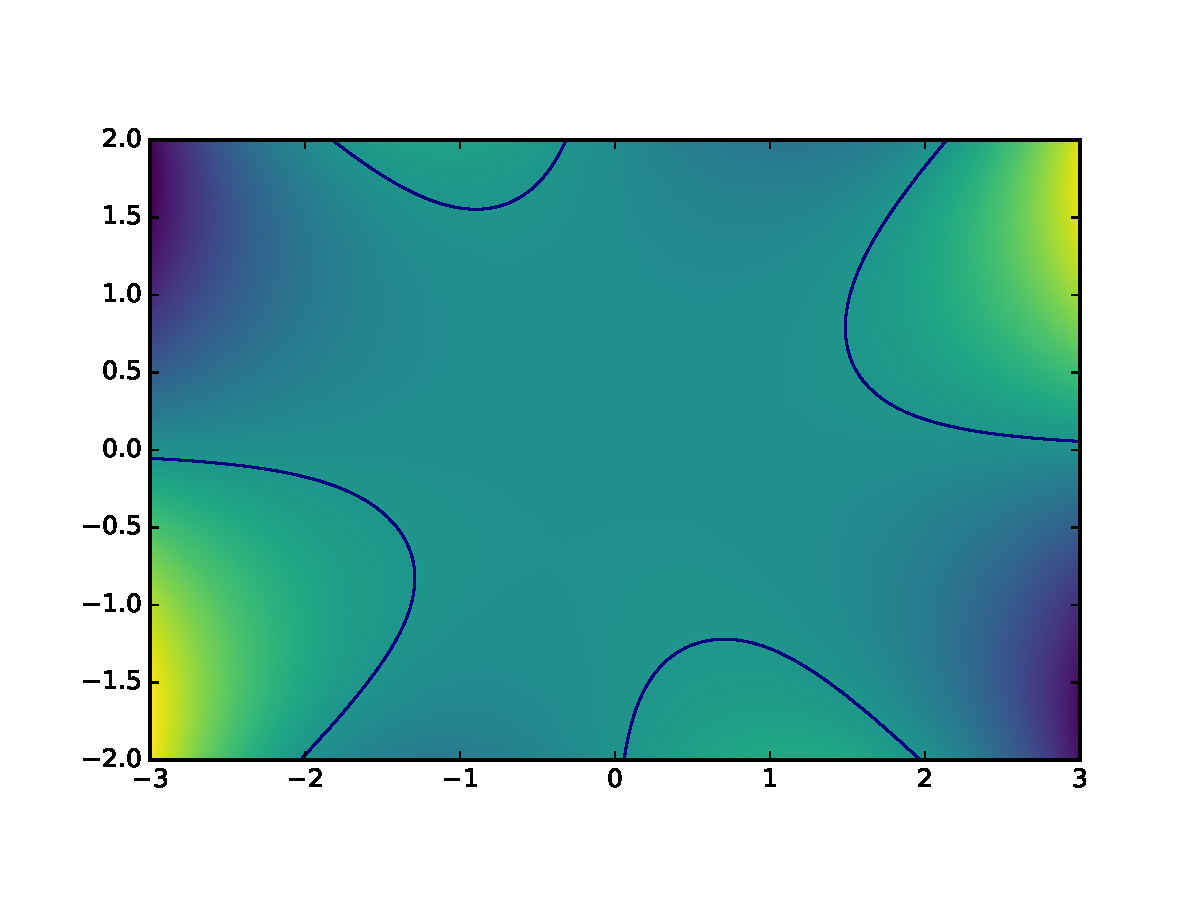
\includegraphics[width=10cm, height=8cm]{img/curva0f2.pdf}
%  \caption{Curva de nivel 0 de $F_{2}$.}
%  \label{fig:sub2}
%\end{subfigure}
%\caption{Curvas de nivel 0 de $F_{1}$ y $F_{2}$}
%\label{fig:test}
%\end{figure}


% ---------------- Comando para hacer itemes
% \Solution{pregunta}{solucion}
\newcommand{\Solution}[2]{%
	\item #1 \vspace{0.2cm}
	\textbf{Soluci\'on:} #2
}
% \Demonstration{pregunta}{demostracion}
\newcommand{\Demonstration}[2]{%
	\item #1 \vspace{0.2cm}
	\begin{proof}
		#2	
	\end{proof}
}

% ---------------- Opciones de algortihm2e
\SetKw{KwRequire}{Require:}

% ---------------- Opciones de background.
\SetBgColor{black}
\SetBgScale{1}
\SetBgOpacity{1}
\SetBgAngle{0}
\SetBgContents{%
	\begin{tikzpicture}[remember picture,overlay]
		\node at (-8.0,0.746\textheight) {
\includegraphics[height=18mm,width= 0.155\textwidth]{img/LogoUIngenieria.png}};
	\end{tikzpicture}
}

% ---------------- Creacion de institucion, departamento y curso.
\fancyheadoffset[L]{-2cm}
\fancyhead[L]{\footnotesize{\textbf{\textsf{Universidad de Chile \\ Facultad de Cs. F\'isicas y Matem\'aticas \\ Departamento de F\'isica \\ FI3104-1: M\'etodos Num\'ericos para la Ciencia e Ingenier\'ia. }}}}
\renewcommand{\headrulewidth}{0pt}
\setlength{\voffset}{-3cm}

\pagestyle{fancy} % Estilo de las páginas

\begin{document}

\pagenumbering{gobble} % Quita el numero de las paginas (y las resetea a 1)

\clearpage

\thispagestyle{fancy}
\vspace*{6.5cm} % Espacio vertical para posicionar bien el título (En una de esas esto se puede optimizar para que no sea tan a la fuerza bruta).

% ---------------- Titulo.
\begin{center}
	\Large{\textbf{\textsf{Tarea $\text{N}^\text{o}$3}}} \\
	\huge{\textbf{\textsf{Interpolaci\'on de Polinomios.}}}
\end{center}

\vspace*{5.5cm}

% ---------------- Integrantes, profes, etc.
\begin{Parallel}{1cm}{7.5cm}
	\ParallelRText{%
		\begin{flushright} % Tira el texto hacia la derecha.
			\large{%
				\textsf{%
					\begin{tabular}{rl}
%						Integrantes: &
%							\begin{tabular}[t]{@{}l@{}}
%								Integrante 1. \\
%								Integrante 2.
%							\end{tabular} \\
						& Jos\'e Ignacio Vines. \\
						Profesor: & 
							\begin{tabular}[t]{@{}l@{}}
						 		Valentino Gonz\'alez.
							\end{tabular} \\
						Auxiliares: &
							\begin{tabular}[t]{@{}l@{}}
								Mario Aguilar. \\
								Ignacio Armijo. \\
								Mar\'ia Constanza Flores. \\
							\end{tabular} \\	
%						Ayudantes: &
%							\begin{tabular}[t]{@{}l@{}}
%								Ayudante 1. \\
%								Ayudante 2.
%							\end{tabular} \\		 
					\end{tabular}
					Fecha: \today
				}
			}
		\end{flushright}
	}
\end{Parallel}

\clearpage

\pagenumbering{arabic} % Numeros de pagina Arabicos (y los resetea a 1)

\newpage

\tableofcontents % Indice. Descomente para usar.
\listoffigures % Lista de figuras. Descomente para usar.
%\listoftables % Lista de tablas. Descomente para usar.

\newpage

\section{Introducci\'on}
El objetivo del presente informe es investigar c\'omo se comportan la interpolaci\'on de polinomios contra la de Spline, y utilizar el m\'etodo de interpolaci\'on de Spline en 2 dimensiones para reparar una imagen da\~nada de una galaxia.

La interpolaci\'on de polinomios consiste en, dado un conjunto de puntos, encontrar un polinomio que pase por estos. Por otro lado, un Spline es una funci\'on definida por tramos de polinomios, con un grado de suavidad en los puntos, o nodos, donde se unen estos.

\section{Procedimiento}
\subsection{Comparaci\'on de M\'etodos}
Para comparar como funcionan los m\'etodos, estos se aplicar\'an a una funci\'on Gaussiana definida como sigue:
\begin{equation}
	f(x) = e^{-x^{2}/0.05}
\end{equation}

En primera instancia se divide el intervalo $[-1,1]$ en 4 tramos equiespaciados con la funci\'on \textbf{linspace}, dejando un total de 5 puntos para llevar a cabo la interpolaci\'on, luego, haciendo uso del m\'odulo \textbf{scipy.interpolate} y de la funci\'on \textbf{lagrange} y clase \textbf{UnivariateSpline} se hace la interpolaci\'on, aumentando en 5 el n\'umero de puntos para la interpolaci\'on hasta llegar a 20, siempre manteniendo el equiespaciado del intervalo.

La funci\'on \textbf{lagrange} recibe como argumentos dos vectores, $x$ e $y = f(x)$: un vector con el intervalo de puntos a samplear y uno con la funci\'on evaluada en dichos puntos respectivamente, y retorna un polinomio de Lagrange que pasa por todos los puntos de $x$. 

La clase \textbf{UnivariateSpline} recibe como argumentos dos vectores, $x$ e $y = f(x)$: un vector con el intervalo de puntos a samplear y uno con la funci\'on evaluada en dichos puntos respectivamente, y como par\'ametros adicionales recibe $s$, un factor de suavidad utilizado para elegir el n\'umero de nudos del Spline, y $k$, el orden del Spline. Se elige $s=0$ para que pase por todos los puntos del intervalo y $k=3$ para que sea un Spline c\'ubico. Esta clase instancia un objeto de tipo \textbf{UnivariateSpline} que representa un Spline que pasa por todos los puntos de $x$.

La clase \textbf{UnivariateSpline} es un wrapper de FITPACK, un paquete de subrutinas escrito en FORTRAN utilizado para calcular Splines suaves para distintos tipos de datos y geometr\'ias\footnote{http://www.netlib.org/dierckx/}; en particular \textbf{UnivariateSpline} hace uso de la subrutina \textbf{fpcurf0}, que a su vez utiliza la subrutina \textbf{fpcurf}\footnote{El archivo fpcurf.f est\'a incluido en la carpeta for\_routines en el repositorio.} para calcular el Spline.
La condici\'on de suavidad que se debe cumplir en los nodos es que la k-\'esima derivada del Spline sea 0. La documentaci\'on de \textbf{fpcurf} no contiene informaci\'on de c\'omo maneja la implementaci\'on los extremos del intervalo, sin embargo la implementaci\'on cl\'asica del m\'etodo de Spline es imponer que la segunda derivada del Spline en los extremos sea 0, as\'i el Spline sigue una l\'inea recta desde los extremos.

\subsection{Reparaci\'on de Imagen}
Para reparar la imagen primero se toma una secci\'on de ella sobre la cual se interpolar\'a un Spline de dos dimensiones

\section{Resultados}

\section{Conclusiones}

\end{document}
